% This is samplepaper.tex, a sample chapter demonstrating the
% LLNCS macro package for Springer Computer Science proceedings;
% Version 2.21 of 2022/01/12
%
\documentclass[runningheads]{llncs}
%
\usepackage[T1]{fontenc}
% T1 fonts will be used to generate the final print and online PDFs,
% so please use T1 fonts in your manuscript whenever possible.
% Other font encondings may result in incorrect characters.
%
\usepackage{graphicx}
% Used for displaying a sample figure. If possible, figure files should
% be included in EPS format.
%
% If you use the hyperref package, please uncomment the following two lines
% to display URLs in blue roman font according to Springer's eBook style:
%\usepackage{color}
%\renewcommand\UrlFont{\color{blue}\rmfamily}
%\urlstyle{rm}
%
\usepackage{amsmath}  % Required for \text command
\usepackage{amssymb}
\usepackage{cleveref}
\usepackage{graphicx}
\usepackage{subcaption}
\usepackage{verbatim}
\begin{document}
%
\title{Contribution Title}
%
%\titlerunning{Abbreviated paper title}
% If the paper title is too long for the running head, you can set
% an abbreviated paper title here
%
\author{Anna Vitali\inst{1}\orcidID{0000-1111-2222-3333} \and
Second Author\inst{2,3}\orcidID{1111-2222-3333-4444} \and
Third Author\inst{1}\orcidID{2222--3333-4444-5555}}
%
\authorrunning{}%{A. Vitali, R. Amadini et al.}
% First names are abbreviated in the running head.
% If there are more than two authors, 'et al.' is used.
%
\institute{Alma Mater Studiorum Università di Bologna, Bolgona, Italy\\
%\url{http://www.springer.com/gp/computer-science/lncs} \and
%ABC Institute, Rupert-Karls-University Heidelberg, Heidelberg, Germany\\
\email{\{anna.vitali7\}@unibo.it}}
%
\maketitle              % typeset the header of the contribution
%
\begin{abstract}
In the manufacturing industry, maintaining the stability of workpieces during operations such as cutting, milling, and contouring is essential to ensuring the quality of the final product. This stability is achieved using fasteners that are strategically placed to minimize vibrations and oscillations. However, determining the optimal positioning of these fasteners, ensuring their safety during cutting operations, and keeping the workpiece securely in place is a complex task, especially when dealing with composite materials that consist of multiple components requiring simultaneous support.

Although modern machining systems offer assistance in determining fastener positions, these suggestions must closely align with the expertise of experienced operators. This paper presents a solution to the fastener positioning problem using Constraint Programming (CP). By capturing and formalizing the knowledge of skilled operators, we demonstrate how CP can be applied to improve upon existing system recommendations. The results show that this approach can reduce errors and enhance the overall stability of the component during manufacturing processes, leading to improved quality and precision in the final product.

\keywords{First keyword  \and Second keyword \and Another keyword.}
\end{abstract}
%
%
%

\section{Introduction}

In manufacturing industry, finding the correct positioning of the parts fasteners during the milling and cutting processes, in order to reduce vibrations and keep the element as firm as possible, is a fundamental problem to be solved to ensure a certain quality of the finished product \cite{fei2020state}.

Several studies have been carried out on the forms and materials of fasteners that can be used to minimize oscillations and vibrations \cite{sivasubramanian2019optimization,chung2001materials}, among these one of the most adopted strategies in the manufacturing field involves the use of adsorption methods based on the adoption of vacuum suction cups \cite{zhu2006principle,del2019thin}.

In this study, we will use as a reference a machine capable of performing operations on a wooden panel, such as milling, contouring, and drilling, supported by a system of movable bars on which suction cups can be vertically adjusted for secure holding. 

Several factors must be taken into account for effective positioning of suction cups, including the type of machining operation, the specific areas of the workpiece that will be affected, and the geometry of the part \cite{rachierumethodology}. In particular, when dealing with cutting operations, it is essential to avoid placing fixtures beneath areas where through-cuts will occur to prevent potential damage to the fasteners.

It is also important to consider that the available resources are limited. Typically, the machine has a fixed capacity, allowing for only a certain number of bars and a finite number of various types of fixings. Within these constraints, we must decide how to allocate the resources efficiently, ensuring that we do not exceed the available quantity while providing adequate support for the workpiece. The objective, however, is not to maximize the use of resources but to strategically cover the most critical areas of the workpiece to achieve optimal support.

To address this problem, we propose a constraint optimization model to decide where to place the bars and on them where the suction cups can be inserted and we compered the results with those generated by the current system. The comparison showed that the solution derived from CP was more straightforward to implement, lowering the risk of human error. In the current system, the machine operator is required to manually determine the number of suction cups to use, which heightens the possibility of mistakes, particularly when an insufficient number is chosen.

Moreover, the CP-based solution demonstrated an improvement in the support of the workpiece. Specifically, the solution ensures that if components are cut from the original piece, each sub-part large enough to accommodate suction cups is adequately supported, thereby preventing its unintended detachment. This is achieved by ensuring that the center of gravity of each sub-part remains within the perimeter formed by the fixtures inside it. In contrast, examples show that some solutions generated by the current system fail to meet this requirement, whereas the CP solution consistently satisfies this condition.

The remainder of this article is organized as follows. Section 2 presents an overview of similar problems that have been addressed using Constraint Programming. In Section 3, we explain the method used to identify the optimal points for support placement and how these points are represented. Section 3 details the constraint model developed to determine the positioning of the elements. Finally, Section 4 presents the results of our approach, comparing them with those of the previous system.

% Section 2 presents an overview of similar problems that have been addressed using Constraint Programming. 



\section{Related works}

In this section, we analyze research on the optimal placement of fasteners and suction cups in manufacturing processes, with a particular emphasis on constraint optimization, vibration reduction, and support during machining operations. Additionally, we present studies addressing positioning problems that have been solved through Constraint Programming (CP), alongside strategies closely related to those implemented in our work.

In the study by Avigal et al. \cite{avigal2022gomp}, the authors investigate suction cup grasping in industrial applications, focusing on the balance between suction forces and motion to prevent detachment. They propose a hybrid optimization approach that integrates deep learning techniques, demonstrating that the learned constraint can allow the solver to speed-up motions. Lee et al. \cite{lee2024grasp} introduce a grasp failure model applicable to various suction cup configurations, highlighting constraints that ensure fast and reliable object manipulation. These constraints have been incorporated into trajectory optimization algorithms and used to address time-optimal trajectory planning. In another study \cite{miriyev2020fastener}, the authors explore optimization techniques for fastener placement under constrained resources in airplane assembly process, proposing and comparing several algorithms.

The problem of determining the optimal positioning of elements with specific characteristics within a defined area has been extensively studied in the literature, particularly within the field of telecommunications \cite{younis2008strategies}. Several studies have addressed the optimal positioning of devices within environments, such as beacons or workstations, to ensure adequate coverage of a specific area, considering the characteristics of devices. These studies often employ Constraint Programming to determine the most effective solution \cite{loffler2022optimal,fruhwirth1998optimal}, and a commonly strategy for modeling such problems involves generating a map of the area of interest, wherein regions are identified as more or less suitable for device placement \cite{loffler2022optimal,fruhwirth1998optimal,vlasenko2014smart}. This approach is highly applicable to our problem and has been adopted in the present study to guide the positioning of fasteners.


\section{Identification of Optimal Fastener Placement Points}

The geometry and surface area of the part must be considered when identifying the optimal fixture points. It is important to recognize that different types of elements may be produced: individual components that do not require further machining to generate additional parts, and composite components, where material is removed from a single element to create the final shape or where multiple components are derived from a single element through machining.

Expert knowledge regarding the proper positioning of suction cups suggests that, for small parts capable of supporting at least one fixture, the central area should be prioritized. For medium-sized parts, it is preferable to focus on the perimeter, while for larger parts, both the perimeter and the center must be adopted for support. To categorize the part size, the relationship between the surface area of the element and the available support area is examined:

\[
	ratio  = \frac{element\_area}{support\_area} 
\]

The proposed solution involves representing the part and the machining process in a matrix, where precision is measured in millimeters to match the machine's accuracy. Each cell in the matrix is assigned a score that reflects the suitability of that specific point for securing a fixture (\cref{fig:scorematrixdashboard}). In the case of composite parts, higher priority is given to the innermost components, resulting in higher scores compared to the outermost elements, thereby favoring their priority. For positioning purposes, the top-left corner of the fixture is used as a reference point, as illustrated in \cref{fig:referencepointbarssuctioncups}, meaning that the solution aims to determine the coordinates of this point while accounting for the spatial dimensions of the part.

\begin{figure}
	\centering
	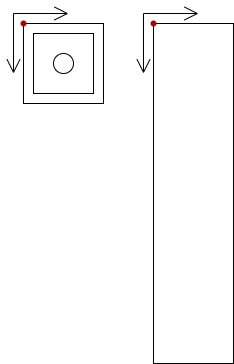
\includegraphics[width=0.2\textwidth]{img/reference_point_bars_suction_cups}
	\caption{Reference point for bar and suction cups positioning}
	\label{fig:referencepointbarssuctioncups}
\end{figure}

The score matrix functions as a map to be utilized by the model in guiding the placement of fixtures. This mapping process allows for the identification of optimal fixture locations, ensuring that constraints related to the geometry of the part are respected. For instance, in the case of a medium-sized circle, the matrix scores are likely to be higher near the center and lower towards the perimeter.

\begin{figure}
	\centering
	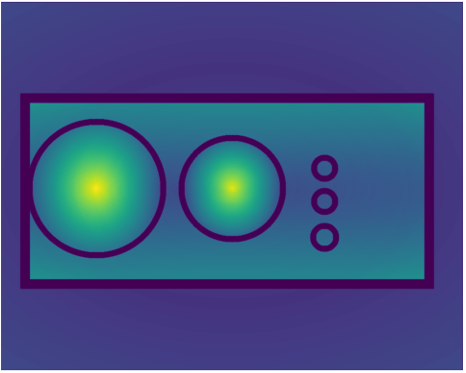
\includegraphics[width=0.4\linewidth]{img/score_matrix_dashboard}
	\caption{Score matrix for a dashboard}
	\label{fig:scorematrixdashboard}
\end{figure}

The \cref{fig:scorematrixdashboard} shows a composite piece (a dashboard) consisting of a medium-sized inner rectangle, so the perimeter is highlighted and five circles for which three of them are too small to be supported and the other two, instead, are considered small, and for them the center is highlighted.


\section{Model}
In this section, we delineate the fundamental components of our model, including the input parameters, variables, constraints, and objective function. The model is characterized as \textit{parametric} because the definitions of the variables, constraints, and objective function are contingent upon the input parameters.

The model developed to establish the positioning of the devices employs the strategy of the Knapsack algorithm
\cite{kellerer2004multidimensional}. Specifically, this problem can be interpreted as a variation of the Geometric Knapsack problem, in which only one dimension of the objects is considered: the width for the bars and the height for the suction cups.

The model is executed iteratively. Initially, it determines the optimal positioning of the bars, and subsequently, based on this, it identifies the placement of the suction cups for each bar.

\subsection{Parameters}
The input parameters are those \textit{constant} values shaping a particular \textit{instance} of the model \cite{wallace2020building}. We formalize them as follows.

\subsubsection{Capacity, Resources and Position}
We define \(\mathsf{capacity}\) as the total space available along the reference axis for the placement of bar or suction cup devices. Additionally \(\mathsf{max\_resources}\) represents the maximum number of bar or suction cups that can be utilized by the machine, while \(\mathsf{max\_position}\) indicates the maximum number of locations available for device insertion. 

We assume that all these values are integers, determined based on the geometry of the workpiece and the resources allocated to the machine. 

The placement of objects must be arranged in such a manner that they do not overlap with one another and do not exceed the available capacity.


\subsubsection{Object and Positions}
Let \(\mathsf{OBJECT} = \{1, \dots,  \mathsf{max\_position}\}\) be the set of objects, and \(\mathsf{POSITION} = \{1, \dots, \mathsf{max\_positions}\}\) be the set of available positions. The size of each object \(i \in \mathsf{OBJECT}\) is given by the function \\\(\mathsf{object\_size} \colon \mathsf{OBJECT} \to \mathbb{N},\) where \(\mathsf{object\_size}[i]\) denotes the size of object \(i\). 

The profit of each position \(j \in \mathsf{POSITION}\) is defined by the function \\\(\mathsf{position\_profit} \colon \mathsf{Position} \to \mathbb{N}\) where \(\mathsf{position\_profit}[j]\) indicates the profit associated with the position \(j\).

The goal of the model is to maximize the total profit resulting form locating objects in the available positions.

\subsection{Variables}

We define the model's primary variable, \(\mathsf{object\_position}[i]\), which indicates the placement of object \(i\) on the axis of interest, where \(\mathsf{object\_position}[i] \in \mathsf{POSITION}\). Each object is either selected or not selected for placement. The selection of object \(i\) is represented by a binary variable \(\mathsf{object\_selected}[i] \in \{0, 1\}\), defined as:

\[
\mathsf{object\_selected}[i] =
\begin{cases}
	1, & \text{if object } i \text{ is selected}, \\
	0, & \text{if object } i \text{ is not selected}.
\end{cases}
\]

This approach allows us to know the number of resources that will be used and for each of them what will be its placement in the workplane, leaving out the resources that will not be allocated.

\subsection{Constraint and Objective}

The idea of Constraint Programming is to solve problems by stating constraints about the problem, and consequently, finding solution satisfying all the constraints. A \textit{constraint} is simply a logical relation among variables, restricting the possible values which they can take \cite{bartak1999constraint}. For our problem we defined the following constraints.

\subsubsection{Capacity Constraint} First of all we need to ensure that the total space occupied by the selected objects does not exceed the available \(\mathsf{capacity}\) which is the width for the bars and the height for the suction cups of the workpiece. This is formalized by the constraint

\[
\sum_{i \in \mathsf{OBJECT}} \mathsf{object\_size}[i] \cdot \mathsf{selected}[i] \leq \mathsf{capacity}
\]

\subsubsection{Non-overlapping Constraint} To avoid overlapping objects, we ensures that the space occupied by the \(i-th\) object, which is specified by \(\mathsf{object\_position}[i]\), if selected does not occupy the position of the next object indicated by \(\mathsf{object\_position}[x + 1]\). This is written as:

\[
(\mathsf{object\_position}[i] + \mathsf{object\_size}[i]) \cdot \mathsf{object\_selected}[i] < \mathsf{object\_position}[i+1] \quad \forall i \in \mathsf{OBJECT}
\]

\subsubsection{Increasing Order Constraint} The increasing order constraint ensures that the positions of the selected objects are in strictly increasing order. This constraint is of interest to obtain the coordinates of elements in ascending order, for correctly represent them later in post-processing, and is captured by the built-in \(increasing\) constraint:

\[increasing(\mathsf{object\_position})\]

\subsection{Objective Function}

The objective function is designed to maximize the profit generated from the strategic positioning of devices. 

The selected object (\(\mathsf{object\_selected}\)) are positioned in specific locations (\(\mathsf{object\_position}\)), each associated with a known profit (\(\mathsf{position\_profit}\)), as a result the objective function becomes:

\[
\max \sum_{i \in \mathsf{OBJECT}} \mathsf{position\_profit}[\mathsf{object\_position}[i]] \cdot \mathsf{object\_selected}[i]
\]

This function ensures that only the selected objects contribute to the overall profit, with the profit being contingent upon their respective placement positions.

\section{Analysis of results}

\begin{figure}[ht]
	\centering
	\caption{Comparing the solution provided by the system with the one obtained through Constraint Programming}
	\label{fig:comparisondashboard}
	
	\begin{subfigure}[b]{0.4\linewidth}
		\centering
		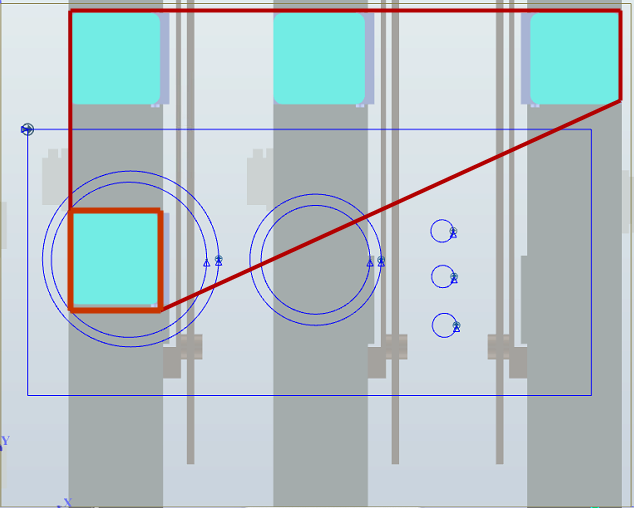
\includegraphics[width=\linewidth]{img/current_system_dashboard_hilighted}
		\caption{Current System Dashboard Solution}
		\label{fig:currentsystemdashboardhighlighted}
	\end{subfigure}
	\hfill % Add horizontal space between subfigures
	\begin{subfigure}[b]{0.4\linewidth}
		\centering
		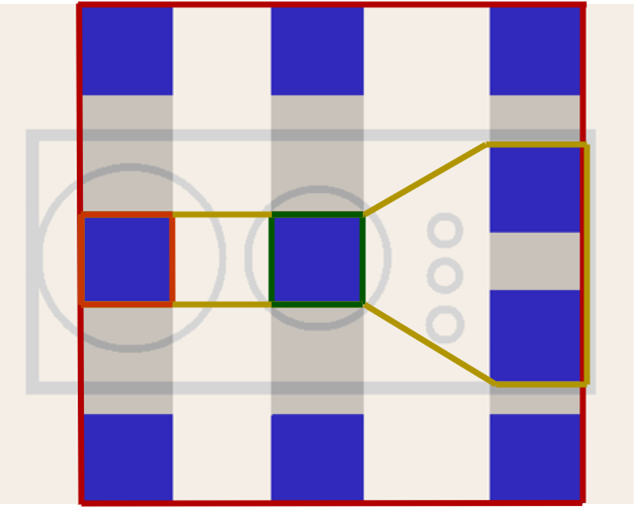
\includegraphics[width=\linewidth]{img/dashboard_cp_system_highlighted}
		\caption{Constraint Programming Dashboard Solution}
		\label{fig:dashboardcpsystemhighlighted}
	\end{subfigure}
\end{figure}

Comparing the results obtained through the solution implemented through Constraint Programming with that of the current system, is noted that the support provided to the workpiece is better, as it is able to comply with the rules stated above, succeeding in case of composite parts to support the elements that must be exported.

The following figure illustrates the solution provided by the system for the dashboard illustrated above. It is evident that the perimeter defined by the suction cups does not sufficiently support either the smaller circle or the inner rectangle. Additionally, the support for the outermost rectangle is critically compromised, as the lower right section lacks fasteners.

In contrast, the solution derived from Constraint Programming demonstrates the successful integration of suction cups that supports both circles, as well as the inner rectangle. The inner rectangle is particularly challenging to support due to its medium size, necessitating a focus on its perimeter and the machining process required to create the circles restricts the available space for fasteners along this. However, the strategic placement of suction cups at the center of the circles provides adequate support for the rectangle, which will be processed first. For further examples, please refer to the appendix.

Finally, the solution obtained through constraint programming can automatically manage the available resources, eliminating the need for the operator to manually specify the number of suction cups required. The necessary quantity is autonomously determined.


%\section{Conclusion}

\begin{comment}


%
% the environments 'definition', 'lemma', 'proposition', 'corollary',
% 'remark', and 'example' are defined in the LLNCS documentclass as well.
%
\begin{proof}
Proofs, examples, and remarks have the initial word in italics,
while the following text appears in normal font.
\end{proof}
For citations of references, we prefer the use of square brackets
and consecutive numbers. Citations using labels or the author/year
convention are also acceptable. The following bibliography provides
a sample reference list with entries for journal
articles~\cite{ref_article1}, an LNCS chapter~\cite{ref_lncs1}, a
book~\cite{ref_book1}, proceedings without editors~\cite{ref_proc1},
and a homepage~\cite{ref_url1}. Multiple citations are grouped
\cite{ref_article1,ref_lncs1,ref_book1},
\cite{ref_article1,ref_book1,ref_proc1,ref_url1}.

\begin{credits}
\subsubsection{\ackname} A bold run-in heading in small font size at the end of the paper is
used for general acknowledgments, for example: This study was funded
by X (grant number Y).

\subsubsection{\discintname}
It is now necessary to declare any competing interests or to specifically
state that the authors have no competing interests. Please place the
statement with a bold run-in heading in small font size beneath the
(optional) acknowledgments\footnote{If EquinOCS, our proceedings submission
system, is used, then the disclaimer can be provided directly in the system.},
for example: The authors have no competing interests to declare that are
relevant to the content of this article. Or: Author A has received research
grants from Company W. Author B has received a speaker honorarium from
Company X and owns stock in Company Y. Author C is a member of committee Z.
\end{credits
}

\end{comment}
%
% ---- Bibliography ----
%
% BibTeX users should specify bibliography style 'splncs04'.
% References will then be sorted and formatted in the correct style.
%
 \bibliographystyle{splncs04}
 \bibliography{bibliography}
%
% \begin{thebibliography}{8}




	
%%%%%%%%%%%%%%%%%%%%%%%%%%%%%%%%%%%%%%%%%%%%%%%%%%%%%%%%%%%%%%%	
	
%\bibitem{ref_article1}
%Author, F.: Article title. Journal \textbf{2}(5), 99--110 (2016)

%\bibitem{ref_lncs1}
%Author, F., Author, S.: Title of a proceedings paper. In: Editor,
%F., Editor, S. (eds.) CONFERENCE 2016, LNCS, vol. 9999, pp. 1--13.
%Springer, Heidelberg (2016). \doi{10.10007/1234567890}

%\bibitem{ref_book1}
%Author, F., Author, S., Author, T.: Book title. 2nd edn. Publisher,
%Location (1999)

%\bibitem{ref_proc1}
%Author, A.-B.: Contribution title. In: 9th International Proceedings
%on Proceedings, pp. 1--2. Publisher, Location (2010)

%\bibitem{ref_url1}
%LNCS Homepage, \url{http://www.springer.com/lncs}, last accessed 2023/10/25
%\end{thebibliography}

\newpage
\appendix

\section{Appendix}
Below we will show some examples of results, comparing the solutions obtained by the current system with those obtained through Constraint Programming.

In this first example, the element to be realized is a stair step. The solution provided by the current system is not wrong but not optimal, as the right suction cup is too high. In the solution obtained through Constraint Programming, on the other hand, the element is considered of medium size and although the number of fixings used is the same as that of the current system, the solution allows the right suction cup to be positioned more toward the center of the height of the workpiece.

\begin{figure}[ht]
	\centering
	\caption{Comparing the solution provided by the system with the one obtained through Constraint Programming}
	\label{fig:comparisonstairstep}
	\begin{subfigure}[b]{0.4\linewidth}
		\centering
		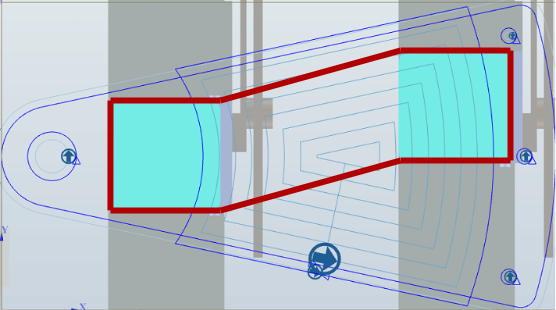
\includegraphics[width=0.7\linewidth]{img/current_system_dashboard_highlighted}
		\caption{Current System Dashboard Solution}
		\label{fig:currentsystemdashboardhighlighted}
	\end{subfigure}
	\begin{subfigure}[b]{0.4\linewidth}
		\centering
		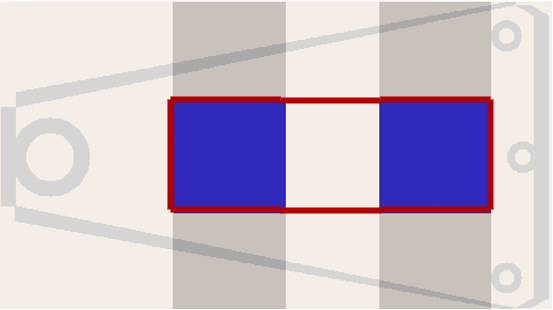
\includegraphics[width=0.7\linewidth]{img/stair_step_cp_highlighted}
		\caption{Constraint Programming Dashboard Solution}
		\label{fig:stairstepcphighlighted}
	\end{subfigure}
\end{figure}


In this example, the creation of a door is required. The solution provided by the system is deemed satisfactory, assuming that the operator accurately inputs the number of suction cups. However, if the operator makes an error in this input, the resulting solution is likely to be incorrect, as evidenced by the lack of support in the center section of the component.

\begin{figure}[ht]
	\centering
	\caption{Comparing the solution provided by the system with the one obtained through Constraint Programming}
	\label{fig:comparisondoor}
	\begin{subfigure}[b]{0.4\linewidth}
		\centering
		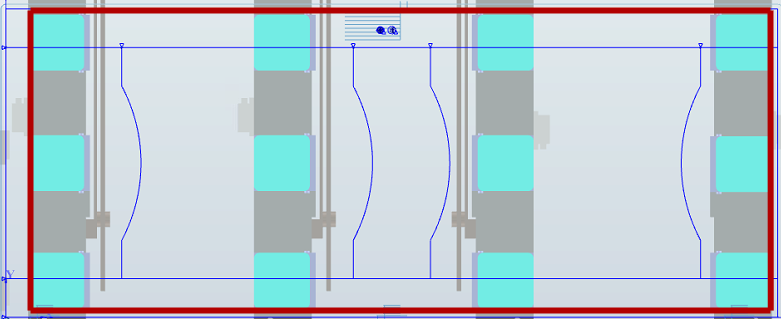
\includegraphics[width=0.7\linewidth]{img/current_system_door_highlighted}
		\caption{Current System Door Solution}
		\label{fig:currentsystemdoorhighlighted}
	\end{subfigure}
	\begin{subfigure}[b]{0.4\linewidth}
		\centering
		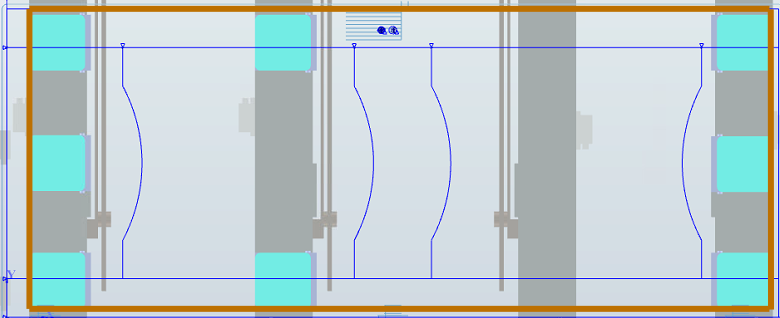
\includegraphics[width=0.7\linewidth]{img/current_system_door_highlighted_bad}
		\caption{Solution with less suction cups}
		\label{fig:currentsystemdoorbadhighlighted}
	\end{subfigure}
	\begin{subfigure}[b]{0.4\linewidth}
		\centering
		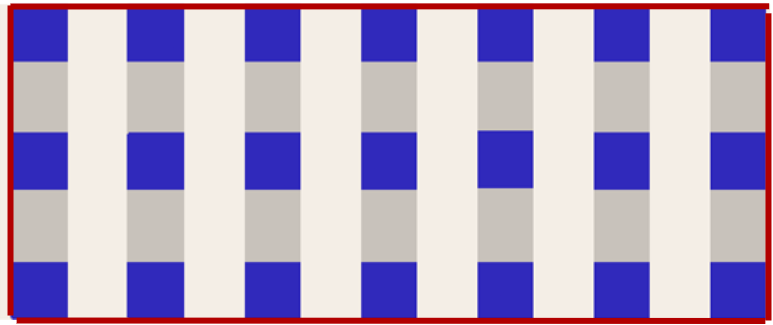
\includegraphics[width=0.7\linewidth]{img/door_cp_highlighted}
		\caption{Constraint Programming Door Solution}
		\label{fig:doorcphighlighted}
	\end{subfigure}
\end{figure}


By employing a constraint-based programming approach, the necessity for manual input of the number of fasteners is eliminated. Consequently, the provided solution will consistently reflect the optimal configuration, thereby mitigating the risk of errors.



\end{document}
